\documentclass[conference]{IEEEtran}
\IEEEoverridecommandlockouts
% The preceding line is only needed to identify funding in the first footnote. If that is unneeded, please comment it out.
\usepackage{cite}
\usepackage{amsmath,amssymb,amsfonts}
\usepackage{algorithmic}
\usepackage{graphicx}
\usepackage{textcomp}
\usepackage{hyperref}
\usepackage{physics}
\usepackage{mathtools}
\usepackage{comment}
\newcommand{\R}{\mathbb{R}}
\newcommand{\Z}{\mathbb{Z}}
\newcommand{\C}{\mathbb{C}}
\newcommand{\Q}{\mathbb{Q}}

\newcommand{\T}{\mathbb{T}}
\newcommand{\p}{\mathcal{P}}
\newcommand{\N}{\mathbb{N}}
\newcommand{\Hilb}{\mathcal{H}}
\newcommand{\Exp}{\mathbb{E}}
\newcommand{\E}{\mathcal{E}}
\newcommand{\w}{\wedge}\usepackage{xcolor}

\def\BibTeX{{\rm B\kern-.05em{\sc i\kern-.025em b}\kern-.08em
    T\kern-.1667em\lower.7ex\hbox{E}\kern-.125emX}}
\begin{document}

\title{Learning with Quantum Computers}


\author{\IEEEauthorblockN{Soham Joshi}
\IEEEauthorblockA{\textit{Computer Science and Engineering} \\
\textit{IIT Bombay (of Aff.)}\\
Mumbai, India \\
sohamjoshi@cse.iitb.ac.in}
}

\maketitle

\begin{abstract}
Quantum Computing (QC), is a developing field with counter-intuitive and surprising results.
Manipulating hidden information caused by the probabilistic nature of quantum information has
enabled researchers to formulate algorithms with lesser asymptotic time complexity\cite{b1}.
Moreover, the combination of hidden information and entanglement at the quantum level has led to 
the reformulation of several machine learning algorithms in the language of quantum computing\cite{b2}.
This survey presents some of the basic concepts needed to understand quantum computing and quantum information, 
and covers some of the machine learning algorithms which have been optimized due to this field.
\end{abstract}

\begin{IEEEkeywords}
Quantum Machine Learning, Quantum Computing, Quantum Information
\end{IEEEkeywords}

\section{Introduction}
This report is a part of the project, ``Machine Learning with Quantum Computers"\cite{b3}, under
the guidance of Siddhant Midha and Aditya Sriram. The project is a part of a program named ``Winter in Data Science'' (WiDS)
conducted by Analytics Club, IIT Bombay. In this paper, basic concepts of quantum computing and quantum information 
will be covered in a way that is accessible to the reader with a knowledge of basic linear algebra and some quantum mechanics.
In this report I will also survey some research papers pertaining to the fields of quantum machine learning (QML). Additionally 
the project includes implementation of quantum algorithms using qiskit and pennylane, the code for which can be found \href{https://github.com/Ihsoj-Mahos/WiDS-QML}{here}.
This paper is meant to be an overview of QC, so some parts of this paper may leave facts without proof. In such cases, kindly refer \cite{b2} for more details.
\section{Quantum bits}
The bit is the fundamental concept of classical computation and classical information. Quantum computation 
and quantum information are built upon an analogous concept, the quantum bit, or qubit for short. Note that 
a bit is just a mathematical entity, in physical circuits high/low voltages can be modelled by a bit taking value
1 or 0. Analogously a qubit is just another abstract mathematical entity. Does this mean that the qubit isn't ``real''?
Yes, a qubit is a tool used for modelling quantum mechanical systems. But studying the properties of the qubit is still 
worth our time since this helps us to develop a theory independent of physical constraints and which helps model reality 
to a good approximation.

\subsection{States of a qubit}
Just as a bit can take values 0, 1; a qubit can be in states $\ket*{0}$, $\ket*{1}$. Moreover, a qubit can be in a linear combination 
of these states given by : 

\begin{equation*}
    \ket*{\psi} = \alpha\ket*{0} + \beta\ket*{1}
\end{equation*}
where $\alpha, \beta \in \C$. \\ 
The state of a qubit is a vector in a two-dimensional complex vector space. The special states $\ket*{0}$ and $\ket*{1}$ are known as 
the computational basis states \footnote{Measurement can be done with respect to a basis other than this. For instance, measurements can be done with respect to the basis $\ket*{+} \equiv \frac{\ket*{0} + \ket*{1}}{\sqrt{2}}, \ket*{-} \equiv \frac{\ket*{0} - \ket*{1}}{\sqrt{2}}$}, form an orthonormal basis for this vector space. 
But, what makes a qubit different from a bit? It is the fact 
that the coefficients of linear combination $\alpha$, $\beta$ cannot be measured. Quantum mechanics tells us that we can obtain much more restricted 
information about this state, particularly, upon measurement, we can obtain $\ket*{0}$ with probability $|\alpha|^2$, and
$\ket*{1}$ with probability $|\beta|^2$. Since the probabilites must sum to 1, the restriction $|\alpha|^2+|\beta|^2 = 1$ is imposed on the
coefficients of linear combination.

\subsection{Bloch sphere}
A tool which helps to visualise actions on a qubit is known as the \textit{Bloch sphere}. Because of the restriction imposed on $|\alpha|, |\beta|$, 
we can rewrite the state of a qubit as : 

\begin{equation*}
    \ket*{\psi} = e^{i\gamma}\left(cos\frac{\theta}{2}\ket*{0} + e^{i\varphi}sin\frac{\theta}{2}\ket*{1}\right)
\end{equation*}
In the next section we will see that global phase factors have no effect so this can be re-written as : 
\begin{equation*}
    \ket*{\psi} = cos\frac{\theta}{2}\ket*{0} + e^{i\varphi}sin\frac{\theta}{2}\ket*{1}
\end{equation*}

\begin{figure}[htbp]
\centerline{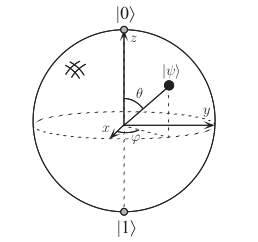
\includegraphics[scale = 0.5]{Images/bloch.png}}
\caption{Bloch sphere representation of a qubit}
\label{bloch}
\end{figure}

\subsection{Multiple qubits}
Suppose we have two qubits. If these were two classical bits, then there would be four
possible states, 00, 01, 10, and 11. Correspondingly, a two qubit system has four computational basis states 
\footnote{Another example of commonly used basis are called the ``bell states'', given by $\ket*{\beta_{00}} = \frac{\ket*{00} + \ket*{11}}{\sqrt{2}}; \ket*{\beta_{01}} = \frac{\ket*{01} + \ket*{10}}{\sqrt{2}}; \ket*{\beta_{10}} = \frac{\ket*{00} - \ket*{11}}{\sqrt{2}}; \ket*{\beta_{11}} = \frac{\ket*{01} - \ket*{10}}{\sqrt{2}}$}
denoted $\ket*{00}, \ket*{10}, \ket*{10}, \ket*{11}$. A pair of qubits can also exist in
superpositions of these four states,
\begin{equation*}
    \ket*{\psi} = \alpha_{00}\ket*{00} + \alpha_{01}\ket*{01} + \alpha_{10}\ket*{10} + \alpha_{11}\ket*{11}
\end{equation*}
Similar to the case for a single qubit, the measurement result x (= 00, 01, 10 or 11) occurs
with probability $|\alpha_x|^2$ , with the state of the qubits after the measurement being $\ket*{x}$.
More generally, we may consider a system of n qubits. The computational basis states
of this system are of the form $\ket*{x_{1}x_{2}{}_{\cdots}x_{n}}$, and so a quantum state of such a system
is specified by $2^n$ amplitudes.

\section{Quantum Gates}
Classical gates are responsible for manipulating bits, essentially representing a boolean function from bits to bits.
Similarly, quantum gates are just a function from qubits to qubits. In this section, we shall explore the different classes of quantum gates. 
We will not delve into proofs but offer an operational description of how quantum gates work.
\subsection{Single-Qubit gates}
A qubit can be written as a $2 \times 1$ unit vector in the space spanned by $\ket*{0}, \ket*{1}$. So, a transformation from a single qubit to 
another qubit transforms a unit vector to another unit vector. Hence, it follows that all quantum gates are unitary. Moreover, it turns out that any 
unitary operation is a valid quantum gate and can be constructed from some ``universal'' quantum gates (will be discussed later).

\begin{figure}[htbp]
\centerline{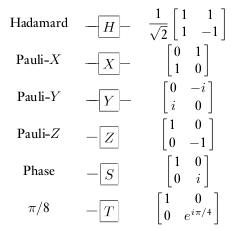
\includegraphics[scale = 0.5]{Images/single-gates.png}}
\caption{Single qubit gates}
\label{singlegate}
\end{figure}

Some single qubit quantum gates are shown in figure \ref{singlegate}. Since we are dealing with the qubit as an abstraction, a quantum gate is just a black box 
operator that performs a unitary transformation to a qubit. For now, we will not deal with the question of the physical realisation of these gates. 

\subsection{Multiple qubit gates}
In classical computation, there are five notable quantum gates, namely \verb|NOT|, \verb|AND|, \verb|OR|, \verb|NAND|, \verb|NOR|. As it turns out, 
all of these gates can be simulated using quantum gates as well. But, as a first step, consider the controlled-NOT, or the \verb|CNOT| gate (figure \ref{cnot}).
Now, we go into an important point when dealing with quantum gates. Even though the circuit diagram shows two input lines in the circuit, the \verb|CNOT| gate doesn't act on 
a single qubit, but a system of two ``entangled'' qubits. Hence, the only correct way to apply the circuit is to take the tensor product of the two input vectors, apply the gate and obtain 
another tensor product. The notation $\ket*{a} \otimes \ket*{b}$ is often abbreviated as $\ket*{a}\ket*{b}$ or $\ket*{ab}$. So the action of a gate $U$ will be given as : 
\begin{equation*}
    \ket*{a}\ket*{b} \xrightarrow[]{U} U\ket*{a}\ket*{b}
\end{equation*}

\begin{figure}[htbp]
\centerline{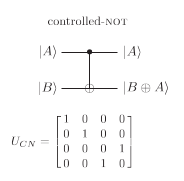
\includegraphics[scale = 0.7]{Images/cnot.png}}
\caption{CNOT gate}
\label{cnot}
\end{figure}

Moreover, just because the control qubit does not change values when it is a computational basis state doesn't mean that it will remain the same for all vectors. In fact, 
the control qubit often changes and measuring it's state is a key step in several quantum algorithms. Another important fact is that 
any multiple qubit quantum gate can be constructed using \verb|CNOT| and single qubit quantum gates. Hence, they form a set of universal quantum gates.
So, the \verb|CNOT| gate is analogous to the \verb|XOR| gate, but not exactly equivalent. Can gates be constructed exactly equivalent to \verb|NAND|, \verb|XOR| gates? Turns out this is 
not possible because quantum gates must be reversible whereas \verb|XOR| and \verb|NAND| gates are irreversible, i.e., given the output of these gates, the input cannot be uniquely identified. 

\subsection{Quantum circuits}
We have already seen some quantum circuits, but let us examine quantum ciruits in some more detail. Each line in the circuit is represented by a wire, but this wire is not necessarily physical, 
it may as well represent the passage of time, or a physical particle such as a photon. There are a few features allowed in classical circuits that are not usually present in
quantum circuits. Loops in a circuit are not allowed, \verb|FANOUT| and \verb|FANIN| operations are not allowed. This is because of the ``no-cloning''\footnote{The no-cloning theorem states that ``qubit-copying'' is not permitted. Hence, junctions of wires are not permitted in a quantum circuit. The no-cloning theorem proves to be useful in quantum encryption protocols like BB84 \cite{b4}} theorem.
An example of a quantum circuit is the ``quantum teleportation circuit''(figure \ref{teleport}). The setting of the problem is that Alice and Bob met long ago but now live
far apart. While together they generated an EPR pair, each taking one qubit of the EPR pair when they separated. Alice now wants deliver a qubit $\ket*{\psi}$ to Bob. She does not know the state of
the qubit, and moreover can only send classical information to Bob. This can be achieved using the circuit given. 

\begin{figure}[htbp]
\centerline{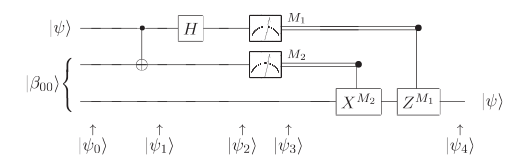
\includegraphics[scale = 0.5]{Images/teleport.png}}
\caption{Quantum circuit for teleporting a qubit. The two top lines represent Alice's system, while the bottom
line is Bob's system. The meters represent measurement, and the double lines coming out of them carry classical
bits (recall that single lines denote qubits)}
\label{teleport}
\end{figure}

\subsection{The Deutsch-Jozsa algorithm}
The problem is as follows. Alice, selects a number $x$ from $0$ to $2^n - 1$, and mails it in a letter to Bob. Bob calculates some function
$f(x)$ and replies with the result, which is either 0 or 1. Now, Bob has promised to use
a function $f$ which is of one of two kinds; either $f(x)$ is constant for all values of $x$,
or else $f(x)$ is balanced, that is, equal to 1 for exactly half of all the possible $x$, and 0
for the other half. Alice's goal is to determine with certainty whether Bob has chosen a
constant or a balanced function, corresponding with him as little as possible. In order to solve this we use the algorithm described (figure \ref{dj-algo}). 
The circuit for the same is shown in figure \ref{dj-ckt}
\begin{figure}[htbp]
\centerline{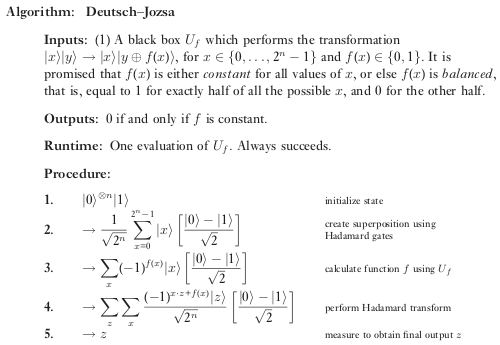
\includegraphics[scale = 0.5]{Images/deutch-algo.png}}
\caption{Deutsch-Jozsa algorithm}
\label{dj-algo}
\end{figure}

\begin{figure}[htbp]
\centerline{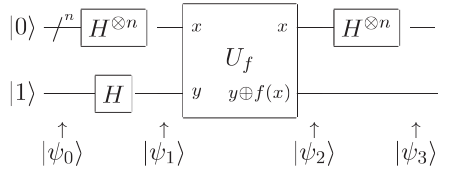
\includegraphics[scale = 0.5]{Images/deutch-ckt.png}}
\caption{Deutsch-Jozsa algorithm's circuit}
\label{dj-ckt}
\end{figure}

Finally, if the measurement yields all 0s then the function is constant, otherwise balanced. The reader can try verifying this as an exercise.

\section*{Acknowledgement}

I would like to thank the mentors of this project Siddhant Midha and Aditya Sriram for giving 
me the opportunity to study and appreciate this subject. 

\begin{thebibliography}{00}
\bibitem{b1} M. Schuld, I. Sinayskiy and F. Petruccione, ``An introduction to quantum machine learning,'' September 2014.
\bibitem{b2} M. Neilson and I. Chuang, ``Quantum Computing and Quantum Information, 10\textsuperscript{th} edition''
\bibitem{b3} S. Midha and A. Sriram ``Learning with Quantum Computers'' \href{https://github.com/siddhant-midha/WiDS-22-Learning-with-quantum-computers-}{\textit{Github repository}}, January 2023.
\bibitem{b4} C. H. Bennett, G. Brassard ``Quantum cryptography: Public key distribution and coin tossing'' March 2020.
\end{thebibliography}
\vspace{12pt}

\end{document}
